

\documentclass[oneside,20pt]{article}          % please do not change
\usepackage[b5paper]{geometry}	    % your paper can be easily printed on a4 or letter paper with enlargenment      
                                    % comment if you have problem with print     
\usepackage{amsfonts,amsmath,latexsym,amssymb}
\usepackage{graphicx}
%%% remove comment delimiter ('%') and specify parameters if required
%\usepackage[dvips]{graphics}

\begin{document}

%%% remove comment delimiter ('%') and select language if required
%\selectlanguage{spanish} 

\noindent 
\begin{center}
  \texttt{LABORATOR 5-- BACKDOOR.}        
\end{center}

\section{SCANAREA UNUI PORT}
\noindent                 
\\\\\
Mai întâi, să aruncăm o privire la scanarea portului. Pachetele pot fi trimise cu diverse protocoale de pe PC-ul hackerului pentru a observa reacția de la PC-ul server. Puteți utiliza diverse protocoale, inclusiv ICMP, TCP, UDP, SCTP etc. De obicei, tehnica de scanare TCP SYN este utilizată în NMap deoarece poate evita cu ușurință detectarea de către dispozitivele de securitate și este, de asemenea, rapidă.
\begin{center}
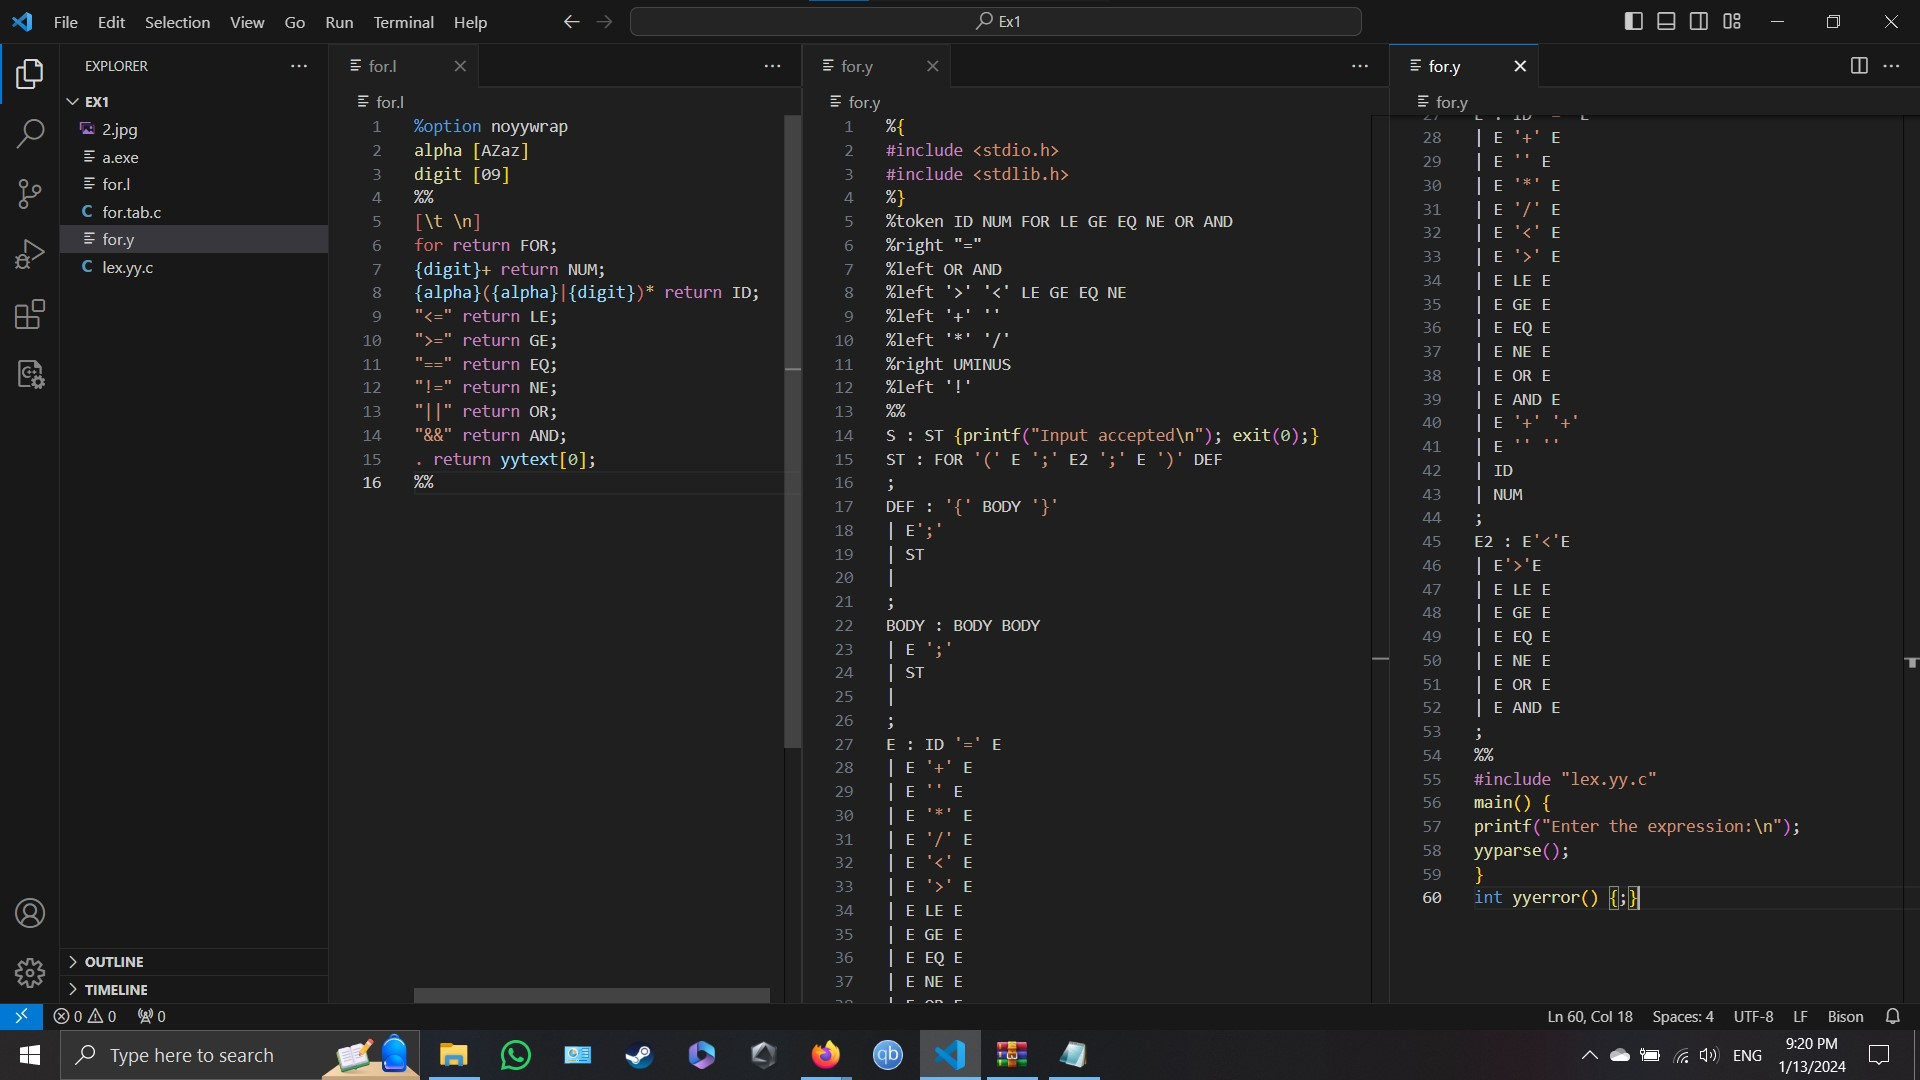
\includegraphics[height=5 cm]{1.png}
\end{center}
Când computerul hacker trimite un pachet TCP SYN la un anumit port al computerului server, computerul hacker primește un pachet ”SYN/ACK” dacă serviciul rulează pe acel port. Dacă portul este închis, ”PC-ul hacker” primește un pachet ”RST”. Când ”PC-ul hacker” primește un pachet ”SYN/ACK”, acesta încheie conexiunea prin trimiterea unui pachet ”RST”. Ca rezultat, scanarea TCP SYN poate fi rapidă și este denumită ”Scanare pe jumătate deschisă”.

  \begin{center}
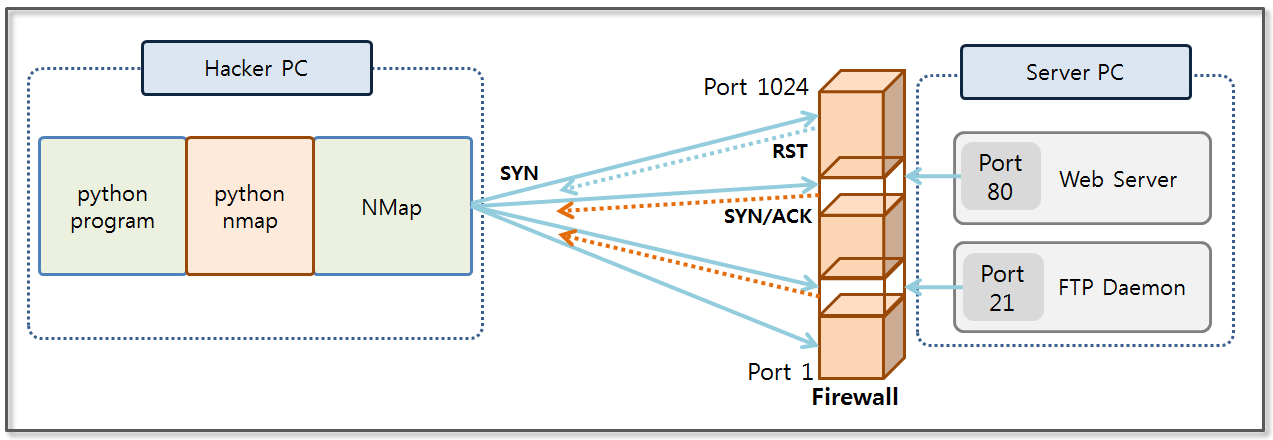
\includegraphics[height=5 cm]{2.png}
\end{center}
Să verificăm de la porturile 1 la 1024 utilizând metoda TCP SYNC SCAN. Un modul socket furnizat de python poate fi folosit pentru a efectua scanarea portului. Cu toate acestea, există un dezavantaj în faptul că acest lucru necesită timp, deoarece este nevoie de timp pentru a aștepta un port fără răspuns. Puteți testa rapid porturile cu modulul NMap. Să aruncăm o privire la un exemplu simplu\\

  \begin{center}
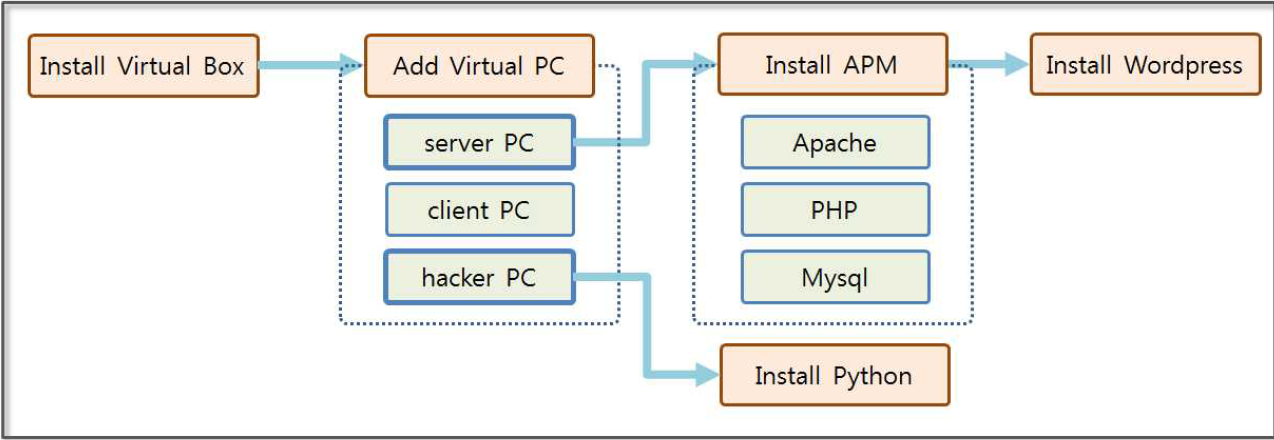
\includegraphics[height=7 cm]{3.png}
\end{center}
Când vine vorba de securitatea informațiilor, chiar și cel mai mic program ar putea fi o bombă cu ceas care așteaptă să primească comenzi de la un atacator pentru a iniția un atac mortal asupra sistemului tău. Programul s-ar putea dovedi a fi o simplă backdoor care inițiază o conexiune la rețeaua atacatorilor așteaptă să primească comenzi și, de asemenea, să poată fura informații.

 

Într-o propoziție, un backdoor este de fapt un software care oferă cuiva acces de la distanță la un computer, de obicei fără permisiunea potrivită atunci când este instalat pe computer. Scopul principal al unei backdoor este de a trimite și primi date, în principal comenzi, printr-un sistem de rețea încoace și încolo.

 

Atacatorul instalează un program rău inocent, care pare să fie un simplu software sau un joc. Odată ce utilizatorul deschide programul, codul backdoor ascuns în program poate iniția o conexiune de la distanță la rețeaua atacatorilor și poate rula orice comenzi date.

 

De asemenea, ar putea să se infiltreze și să ruleze în procesul de fundal, așa că nu mai are nevoie să deschideți programul pentru a iniția o conexiune.


Indiferent cât de conștient de securitate PC-ului este utilizatorul, dacă cineva îl poate păcăli deschizând programul greșit, ajunge ca acesta să compromită și să obțină acces la sistemul utilizatorului de la distanță.

 

În cele ce urmeaza, vom construi un program simplu backdoor în Python și vom arăta cum îl putem folosi pentru a exploata sistemul utilizatorului.


\textbf{Notă: Acesta este doar în scopuri educaționale, nu îl utilizați împotriva niciunei persoane pentru operațiuni ilegale.}\\


\subsection{Noțiuni de bază}
Pentru a începe, trebuie să aveți Python instalat și rulat pe computer. 


Când construiți un "BACKDOOR", sunt necesare două componente:\\

 
\textbf{Client:} Acestea sunt componentele care vor fi instalate pe computerul victimei, inițiază o conexiune la rețeaua atacatorilor, acceptă comenzi și trimite date încoace și încolo.\\
\textbf{Server:} Aceasta este componenta care va fi instalată pe sistemul atacatorului acționând ca punct de intrare ascultând conexiunea client, acceptând conexiunea dacă este de la victimă, trimițând comenzi și primind date.
 

Pentru ca acest lucru să funcționeze, vom folosi modulul Socket care vine încorporat în Python. Modulul socket este folosit pentru a trimite date/mesaje încoace și încolo printr-o rețea. În acest caz, serverul va trimite comenzi (mesaje), clientul primește un mesaj (comenzi), trimite un răspuns (date) și invers.

Deci vom construi două componente: client.py și server.py.
Construiți componenta client
După cum sa explicat mai devreme, componenta client este responsabilă pentru inițierea conexiunii, apoi așteptarea comenzilor din rețeaua atacatorului, rularea comenzii și trimiterea înapoi a unui răspuns, de obicei, rezultatul rulării comenzii.\\
Deschideți client.py:
  \begin{center}
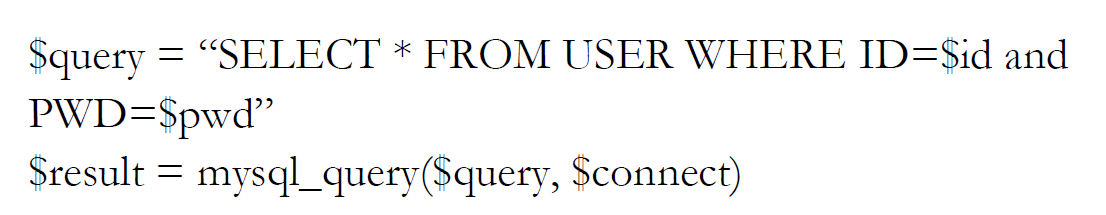
\includegraphics[height=5 cm]{4.png}
\end{center}
Privind codul de mai sus:


Am importat modulele pe care le vom folosi – modulul socket (inițialând conexiunea la rețea) și subprocesul (pentru rularea comenzilor în shell)
Am declarat atacatorii (nostru) telecomandă REMOTE HOST și REMOTE PORT. Ar trebui să actualizați REMOTE HOST cu IP-ul sau localhost – 127.0.0.1. Puteți obține IP-ul dvs. aici.
Am creat conexiunea socket pentru client și am conectat-o ​​la serverul nostru REMOTE.
Apoi am adăugat o buclă while, care continuă să asculte și să aștepte mesaje sau comenzi.
Am extras mesajul din .recv(1024), l-am decodat într-un șir și l-am transmis programului de subproces responsabil cu rularea comenzii.
După rularea comenzii, verificăm atât ieșirea, cât și eroarea, apoi le trimitem pe ambele prin rețea.
Cu asta componenta Client este instalata.
Acum componenta Server:\\

Componenta server este responsabilă pentru ascultarea oricărei conexiuni de intrare de la componenta clientului, acceptarea conexiunii, trimiterea de mesaje (comenzi) și primirea datelor.
  \begin{center}
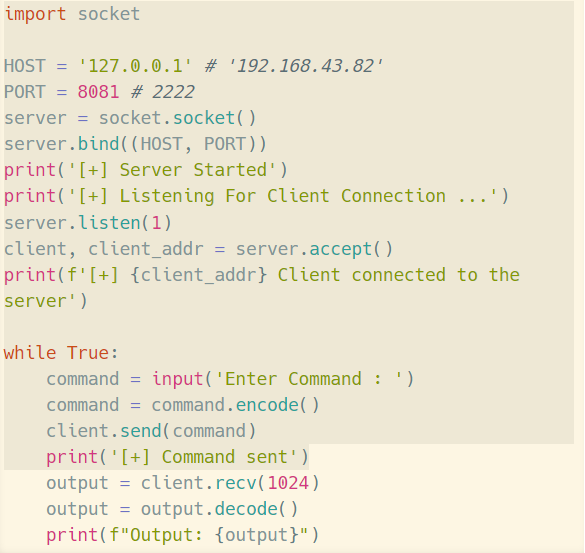
\includegraphics[height=5 cm]{5.png}
\end{center}
Privind codul de mai sus:

Am importat modulul priză (socket) (pentru ascultarea și acceptarea conexiunii la rețea)\\
Ne-am declarat HOST și PORT. Ar trebui să actualizați HOST-ul cu IP-ul sau localhost – 127.0.0.1. Puteți obține IP-ul dvs. aici.\\
A creat conexiunea socket, ascultând conexiunea de intrare și acceptând, dacă există (când utilizatorul rulează programul).\\
Am creat o buclă while pentru a menține conexiunea între componentele client și server.\\
De aici putem cere apoi atacatorului să introducă o comandă, să trimită comanda și să primească un răspuns trimis de componenta client.\\


Testarea programului nostru Backdoor
Odată ce ați creat cu succes cele două componente, acum avem un software simplu backdoor scris cu Python\\
Pentru a testa acest lucru, va trebui să rulați cele două componente simultan și conectate la același HOST și PORT.\\
Deschideți două terminale sau linie de comandă și apoi executați fiecare comandă pe fiecare terminal.\\
Server: python server.py\\
Client: python client.py\\
  \begin{center}
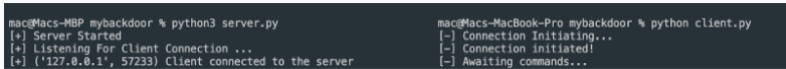
\includegraphics[height=2 cm, width= 12 cm]{6.png}
\end{center}
Dacă vedeți imaginea de mai sus, atunci atât serverul, cât și clientul sunt conectați și așteaptă să trimită și să primească mesaje.\\

Serverul este pregătit să trimită comenzi în timp ce clientul este pregătit să primească comenzi, să îl ruleze și să trimită înapoi rezultatul său.\\

Acum să introducem această comandă în terminalul serverului: echo Hello World:\\
\begin{center}
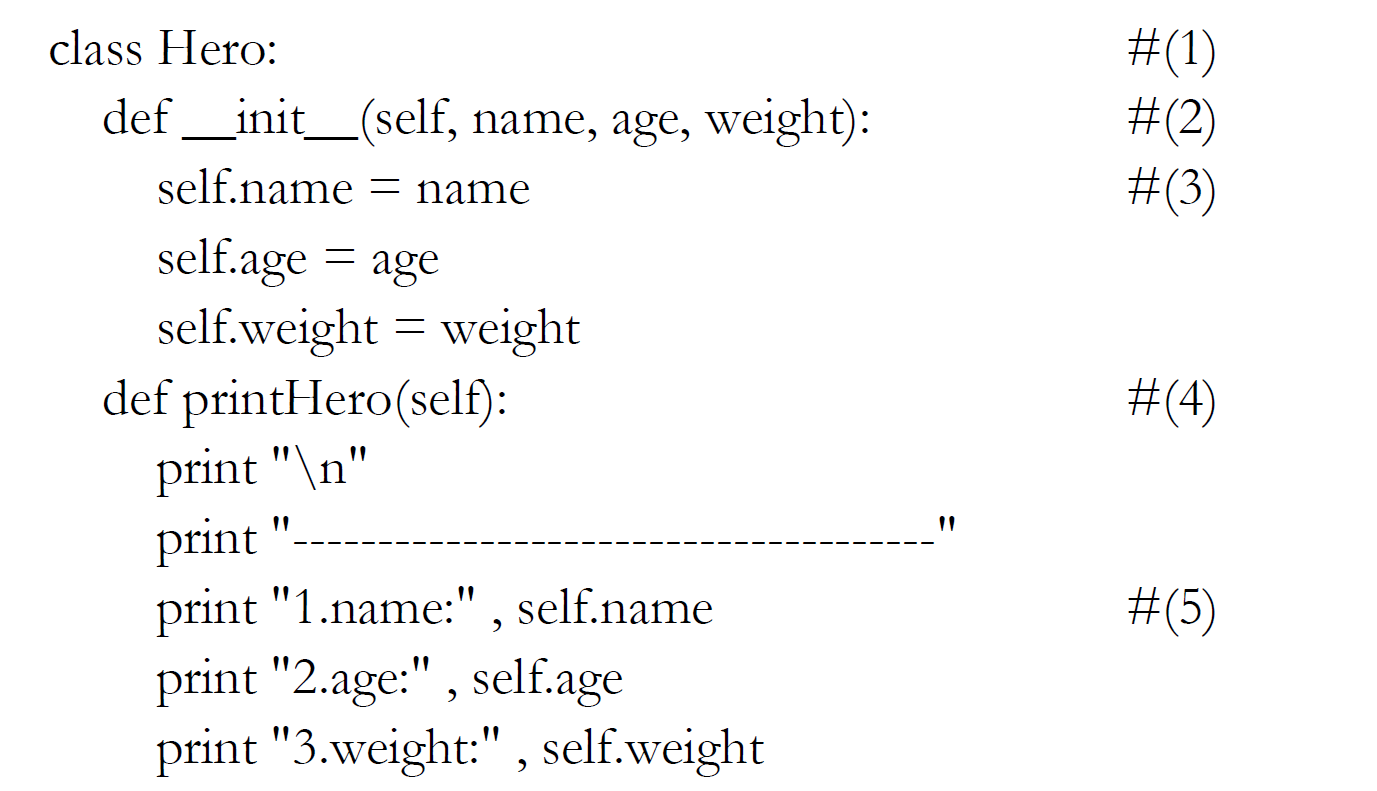
\includegraphics[height=3 cm, width= 12 cm]{7.png}
\end{center}
Ar trebui să vedeți ceva ca imaginea de mai sus. Am trimis comanda echo Hello World, ceea ce înseamnă că ar trebui să imprime Hello World în terminal. Clientul primește această comandă, o rulează și trimite înapoi un răspuns care este rezultatul comenzii.
Să încercăm altul ca: $ls -a ~, cat ~/.aws/config$.
Hopa! Puteți fura literalmente cheia de acces AWS și access_id ale utilizatorului fără ca acesta să știe. Nu numai asta, poți rula și să faci tot felul de lucruri cu acest program simplu backdoor.

 

Cu aceasta, putem concluziona că am compromis computerul utilizatorului și că suntem capabili să obținem acces la computerul utilizatorului și să furăm date.

 

Protejează-te împotriva atacurilor din spate
Aceste tipuri de programe sunt foarte greu de detectat și de protejat, deoarece sunt ascunse departe de vedere și control.

 

Au existat o mulțime de știri despre modul în care oamenii au descoperit ușile din spate în diferite programe pentru programe de utilizator, proiecte open source și chiar organizații mari de software. Ușile din spate pot fi injectate în orice fel de programe, indiferent de sistemul de operare utilizat.

 

Ușile din spate sunt puternic construite pe sistemul de rețea pentru a iniția conexiunea de la distanță cu atacatorul, așa cum am văzut în programul creat mai devreme. Majoritatea sistemelor de operare au firewall-uri care monitorizează orice trafic neobișnuit și suspect încoace și încolo. Cu toate acestea, uneori, firewall-urile nu reușesc să detecteze ușa din spate din cauza modului în care ușile din spate își trimit traficul de rețea, la fel cum s-ar conecta browserele sau alte aplicații la internet.

 

Pentru a preveni acest lucru, puteți crea politici în firewall și puteți alege ce programe doriți să aveți acces la internet și orice alt trafic este blocat. Pentru companii, acestea pot crea politici și pot decide selectiv ce dispozitiv și aplicație are acces la internet.

 

Acest lucru reduce șansa de a avea un software pe care abia îl utilizați, care să servească drept gateway backdoor pentru a vă fura datele.

 

De asemenea, cel mai bun mod de a vă proteja este să nu aveți încredere în niciun software, deoarece majoritatea software-ului este injectat cu cod backdoor fără știrea dezvoltatorilor. Unele dintre aceste aplicații sunt injectate de unele dintre pachetele și dependențele utilizate în construirea aplicației.

 

Aceste dependențe ar putea fi open source și au deja un backdoor. Deci, orice software care utilizează dependențele din software-ul lor are deja un backdoor în programul lor fără ca ei să știe.\\
Deci, aveți încredere zero pentru orice software.\\

 

\section{Concluzie}
În acest laborator, am explicat ce este un Backdoor și cum să construim una. Aceste tipuri de programe sunt o mare amenințare, deoarece este greu să le detectezi, deoarece sunt ascunse într-un program simplu și pot arăta ca un software normal. Majoritatea programelor backdoor sunt incluse ca .dll în Windows sau binare sau ambalate în cadre Python GUI precum Kivy.

Nu utilizați acest lucru pentru a obține acces nedorit la orice computer fără permisiune, deoarece este ilegal. Nu utilizați acest program din motive ilegale, chiar dacă este în cea mai simplă formă.
\section{Bibliografie}

https://www.securecoding.com/blog/how-to-build-a-simple-backdoor-in-python/


\end{document}
